\documentclass[twocolumn]{iob_pb}

%Params
%\def\XILINX{1}
%\def\INTEL{1}

\usepackage{color,soul}
%\usepackage{array}
\usepackage{float}
\usepackage{makecell}

\usepackage[table,xcdraw]{xcolor}
\usepackage{calc}
\graphicspath{{./}{./figures/}}

%\usepackage[showframe]{geometry}% http://ctan.org/pkg/geometry
%\usepackage{lipsum}% http://ctan.org/pkg/lipsum
\usepackage{multicol}% http://ctan.org/pkg/multicols

\definecolor{iob-green}{rgb}{0.0,1.0,0.80}
\definecolor{iob-blue}{rgb}{0.90196,0.94902,1}

\title{IOb-SoC}
\category{IObundle System-on-Chip Platform}
\confidential{}

\usepackage{eso-pic}
\newcommand\BackgroundPic{%
\put(0,0){%
\parbox[b][\paperheight]{\paperwidth}{%
\vfill
\centering

\includegraphics[width=\paperwidth,height=\paperheight,%
keepaspectratio]{bg.png}%
\vfill
}}}


\begin{document}
\AddToShipoutPicture*{\BackgroundPic}

\section*{\textcolor[rgb]{0,0,0}{Overview}}

IOb-SoC is a RISC-V-based System-on-Chip Platform written in Verilog, which
users can download for free, modify, simulate and implement in FPGA or ASIC. It
supports stand-alone and boot loading modes, and can use an internal RAM or an
external DDR controller via an L1/L2 cache system. The IP is currently supported
in ASICs and FPGAs. Licensable commercial versions are available.

\section*{\textcolor[rgb]{0,0,0}{Features}}
\begin{itemize}
\item 32-bit RISC-V control CPU
\item Support for Integer (I), atomic (A) and multiply/divide extensions (M)
\item Instruction and data caches
\item RS232 interfaces for viewing runtime messages
\item Optional timer peripheral
\item Optional Ethernet peripheral
\item Frequency of operation at 167MHz on FPGA
\item Needs external DDR4 memory controller IP
\end{itemize}

\section*{\textcolor[rgb]{0,0,0}{Benefits}}
\begin{itemize}
\item Compact hardware implementation
\item Can fit in low cost FPGAs
\item Can fit in small ASICs 
\item Very low power consumption
\end{itemize}


\section*{\textcolor[rgb]{0,0,0}{Deliverables}}
\begin{itemize}
\item HDL source code
\item Software C source code
\item Simulation testbench
\item Implementation constraints for map, place and route
\item Demo files for commercial FPGA board with Ethernet connectivity
\item User documentation for system integration
\end{itemize}
\newpage

\section*{\textcolor[rgb]{0,0,0}{Block Diagram}}

\begin{figure}[H]
  \begin{center}
    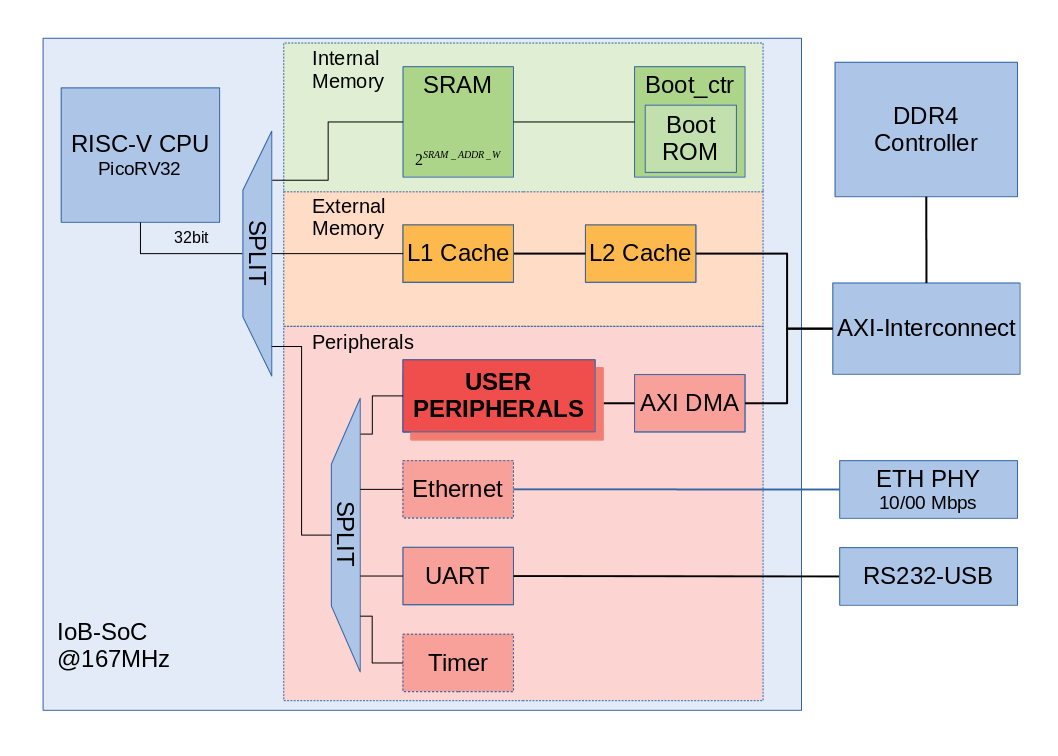
\includegraphics[width=8.5cm]{IoB-SoC_block_diagram.png}
    \caption{IOb-SoC high-level block diagram}
    \label{fig:IOb-SoC}
  \end{center}
\end{figure}


% Please add the following required packages to your document preamble:
% \usepackage[table,xcdraw]{xcolor}
% If you use beamer only pass "xcolor=table" option, i.e. \documentclass[xcolor=table]{beamer}


\section*{FPGA Resources}

\ifnum\XILINX=1
\begin{table}[H]
  \begin{center}
    \begin{tabular}{|l|r|}
      \hline
%      \input xil_results.tex
      \rowcolor{iob-green}
      \textbf{Resource}  & \textbf{Used} \\
      \hline
      \hline

      \input xil_results.tex 

    \end{tabular}
    \caption{Implementation Resources for Xilinx Kintex Ultrascale Devices (with ROM, RAM, L1/L2 caches, DDR controller and UART)}
    \label{tab:res-xil}
  \end{center}
\end{table}
\fi


\ifnum\INTEL=1
\begin{table}[H]
  \begin{center}
    \begin{tabular}{|l|r|}
      \hline

      \rowcolor{iob-green}
      \textbf{Resource}  & \textbf{Used} \\
      \hline
      \hline

      \input alt_results.tex 
        
    \end{tabular}
    \caption{Implementation Resources for Intel Cyclone V Devices (with ROM, RAM, UART)}
    \label{tab:res-alt}
  \end{center}
\end{table}
\fi

\vspace*{0.5cm}
\noindent
\begin{scriptsize}
Disclaimer: IObundle reserves the right to modify the current
technical spe-cifications without notice.
\end{scriptsize}
\newpage


\end{document}
